%%% Method.Rnw --- 

%% Author: emanuelheitlinger@gmail.com

\documentclass[12pt,a4paper]{article}
\usepackage[debugshow,final]{graphics}
\usepackage{hyperref}
\usepackage{float}
\usepackage{lscape} 
\usepackage{rotating} 
 

\date{}
\usepackage{/usr/local/lib64/R/share/texmf/tex/latex/Sweave}
\begin{document}
% make the plots modest size
\title{The transcriptome of A.crassus: Evaluating a method of combining assemblies}
\author{Emanuel Heitlinger}

\maketitle



\section{Overview}
\label{sec:overview}

The pre-processed \textit{A. crassus} data-set consisting of
100491819 bases in 353055 reads (58617
generated using ``FLX-chemistry'', 294438 using
``Titanium-chemistry'') was assembled following an approach proposed
by \cite{pmid20950480}: two assemblies were generated, one using
Newbler v2.6 \cite{pmid16056220}, the other using Mira v3.2.1
\cite{miraEST}. The resulting assemblies (referred to as first-order
assemblies) were merged with Cap3 \cite{Cap3_Huang} into a combined
assembly (referred to as second-order assembly).


\section{The Newbler first-order assembly}
\label{sec:new-fist}




During transcriptome-assembly (with options -cdna -urt) Newbler can
split individual reads spanning the breakpoints of alternate isoforms,
to assemble e.g. the first portion of the reads in one contig, the
second portion in two different contigs. Later multiple so called
isotigs would be constructed and reported, one for each putative
transcript-variant. While this approach could be helpful for the
detection of alternate isoforms, it also produces short contigs
(especially at error-prone edges of high-coverage transcripts) when
the building of isotigs fails. The read-status report and the assembly
output in ace-format the program provides are including short contigs
only used during the assembly-process, but not reported in the
contigs-file used in transcriptome-assembly projects
(454Isotigs.fna). Therefore to get all reads not included in contigs
(i.e. a consistent definition of ``singleton'') it was necessary to
add all reads appearing only in contigs not reported in the fasta-file
to the reported singletons. The number of singletons increased in this
step form the 26211 reported to
109052. We later also address the usefulness of
Newbler's report vs. the expanded singleton-category, but for the
meantime we define singletons as all reads not present in a given
assembly.

\newpage
  

\begin{figure}[H]
  \centering
  
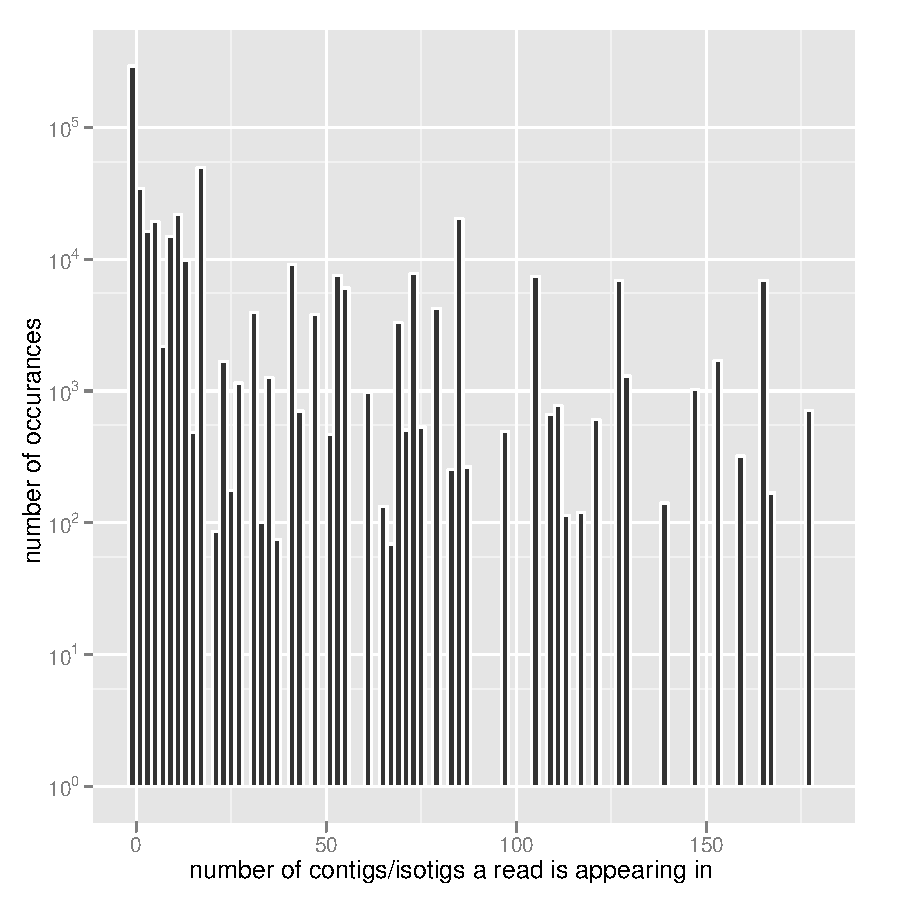
\includegraphics{Method-008}

\caption{A histogram of the number of contigs/isotigs Newbler splitted
  one read into.}
  \label{fig:newdist}
\end{figure}

As mentioned above, the splitting of reads in the Newbler assembly can
give useful information on possible isoforms, however, the number of
contigs \texttt{Newbler} split one read into (in some cases more than
100 contigs) seems artificially inflated (see figure
\ref{fig:newdist}). If information would correspond to real isoforms
it should be about an order of magnitude lower. This fact emphasises
the need for further processing of the contigs. The maximum number of
read-splits in a given contig and its usefulness will be discussed
later in greater detail.

\section{The Mira-assembly and the second-order assembly}
\label{sec:assembly-sec}

The Mira assembly (with options --job=denovo,est,accurate,454)
provided a second estimate of the transcriptome. In this assembly
individual reads are not split. The number of reads not used in the
Mira-assembly was 65368.

To combine the two assemblies Cap3 was used with default parameters
and including the quality information from first-order assemblies. The
reminder of this text deals with the exploratory analysis of how
information from both estimates of the transcriptome are integrated
into the final second-order assembly.

% latex table generated in R 2.14.0 by xtable 1.6-0 package
% Fri Jan 13 08:43:42 2012
\begin{table}[ht]
\begin{center}
\begin{tabular}{rrrr}
  \hline
 & Newbler & Mira & Second-order(MN) \\ 
  \hline
Max length & 6300 & 6352 & 6377 \\ 
  Number of contigs & 15934 & 22596 & 14064 \\ 
  Number of Bases & 8085922 & 12010349 & 8139143 \\ 
  N50 & 579 & 579 & 662 \\ 
  Number of congtigs in N50 & 4301 & 6749 & 3899 \\ 
  non ATGC bases & 375 & 29962 & 5245 \\ 
  Mean length & 508 & 532 & 579 \\ 
   \hline
\end{tabular}
\caption{Basic statistics for the first-order assemblies and the second-order assemly (for which only the most relieable category of contigs is shown 
ef{sec:data-categ-second})}
\label{tab:pc}
\end{center}
\end{table}
Table \ref{tab:pc} gives basic summary-statistics of the different
assemblies. Mira clearly produced the biggest assembly, both in terms
of number of contigs and bases), the second-order assembly is slightly
smaller size than the Newbler assembly.  The second-order assembly had
on average longer contigs than both first-order assemblies and a
higher weighted median contig size (N50).



\newpage
\section{Data-categories in the second-order assembly}
\label{sec:data-categ-second}

Three main categories of assembled sequence data can be distinguished
in the second-order assembly, each one with different reliability and
purpose in downstream applications:

The first category of data obtained are the singletons of the final
second-order assembly. It comprises raw sequencing reads that neither
of the first-order assemblers used. It is therefore the intersecion of
the Newbler-singletons (as defined in \ref{sec:new-fist}) and the
Mira-singletons. 47669 reads fell in this category. A
second category of sequence contains the first-order contigs, that
could not be assembled in the second-order assembly (the singletons in
the Cap3-assembly; M\_1 and N\_1 in table
\ref{tab:categ}). Furthermore second-order contigs in which
first-order contigs from only one assembler are combined (M\_n and
N\_n in table \ref{tab:categ}) also have to be included in this
category. Sequences in this category should be considered only
moderately reliable as they are supported by only one assembly
algorithm.

Finally the category of contigs considered most reliable contains all
second-order contigs with contribution from both first-order
assemblies (MN in table \ref{tab:categ}).

% latex table generated in R 2.14.0 by xtable 1.6-0 package
% Fri Jan 13 08:43:51 2012
\begin{table}[ht]
\begin{center}
\begin{tabular}{rlllll}
  \hline
 & M\_1 & M\_n & MN & N\_n & N\_1 \\ 
  \hline
Snd.o.con &   & 164 & 13887 & 13 &   \\ 
  Fst.o.con & 2347 & 897 & mira=19352/Newbler=14410 & 40 & 1484 \\ 
  reads & 42172 & 21153 & one=269868/both=193308 & 1538 & 13100 \\ 
   \hline
\end{tabular}
\caption{\small{\textbf{Number of reads, first-order contigs (Fst.o.con) and second-order contigs (Snd.o.con) for different categories of contigs (M\_1 and N\_1 = first-order contigs not assembled in second-order assembly, from mira and newbler respectively; M\_n and N\_n =  assembled in second-order contigs only with contigs from the same first-order assembly; MN = assembled in second-order contigs with first order contigs from both first order assemblies}}}
\label{tab:categ}
\end{center}
\end{table}
For this last, most reliable (MN) category, reads contained in the
assembly can be categorised depending on whether they entered the
assembly via both or only via one first-order assembly.

\newpage

\begin{figure}[H]
  \centering
  

\includegraphics{Method-014}

  \caption{The way of reads into the most reliable (MN) assembly-category}
  \label{fig:venncat}
\end{figure}

Figure \ref{fig:venncat} gives a more detailed view of the fate of the
reads Newbler splited during first-order assembly. Interestingly most
reads Newbler splited ended in the high-quality category of the second
order assembly.

\section{Contribution of first-order assemblies to second-order contigs}
\label{sec:contr-firs-order}

  

Looking at the contribution of contigs from each of the assemblies to
one second-order contig in figure \ref{fig:rcp}a it becomes clear,
that the Mira-assembly had a high number of redundant contigs. These
were assembled into the same contig by Newbler and finally also in one
second-order contig by Cap3.


\begin{figure}[H]
  \centering

\includegraphics{Method-018}


\caption{Number of first-order contigs from both first-order
  assemblies for each second order contig (a) number of reads through
  Newbler and Mira for each second-order contig (b)}
\label{fig:rcp}
  
\end{figure}


A different picture emerges from the contribution of reads through
each of the first-order assemblies (figure \ref{fig:rcp}b).  Here, for
most second-order contigs many more reads are contributed through
Newbler-contigs. This is because Newbler has more reads summed over
all contigs caused by the duplication due to the splitting of reads.

\newpage

\section{Evaluation of the assemblies}
\label{sec:eval-three-assembl}


To further compare assemblies (Mira or Newbler first-order assemblies
including or excluding their singletons) and the second-order assembly
(including different contigs-categories and singletons) we evaluated
the number of bases or proteins their contigs and singletons
(partially) cover in the related model-nematodes,
\textit{Caenorhabditis elegans} and \textit{Brugia malayi}. To this
purpose we used Blast (blastx e-value cut-off 1e-5) and a custom
perl-script provided by S. Kumar.

In addition, the size of the assembly can give an indication of
redundancy or artificially assembled data. If it increases without
improving the reference-coverage the dataset is likely to contain more
redundant or artificial information, a more parsimonious assembly
should be preferred.



The database-coverage for the two reference species can then be
plotted against the size of the assembly-dataset to estimate the
completeness conditional to the size of the assembly (figures
\ref{fig:basecov}, \ref{fig:protcov}, \ref{fig:prot80cov}).

From the assemblies excluding singletons (in the lower left corner
with lower size and database-coverage) the highly reliable
contig-category of the second-order assembly produced the highest
per-base coverage in both reference-species, with the Newbler assembly
on a second place and Mira producing the lowest
reference-coverage. When adding the contigs considered lower quality
supported by only one assembler to the second-order assembly the
reference-coverage increased moderately.

Including singletons the Mira and Newber assemblies were of increased
size. A comparison of the Newbler's reported singletons with all
singletons addet to the Newbler-assembly shows, that the reported
singletons increased reference-coverage to the same amount than all
singletons, while the non-reported singletons only increased the size
of the assembly. It can be concluded, that the latter contain hardly
any additional information but only error-prone or variant reads.

The second-order assembly including the intersection of first-order
singletons performed similar to the Newbler assembly for the number of
bases coverd, but was larger in size. Adding the less reliable set of
one-assembler supported second-order-contigs the assembly coverd the
most bases in both references. When not the singleton of the
second-order assembly (as defined in \ref{sec:new-fist}) but the
intersection of Newbler's ``reported singletons'' and Mira's
singletons were considered a very parsimonious assembly with high
reference-coverage (termed fullest assembly; and labeled FU in the
plots above) was obtained.

\begin{figure}[H]

\includegraphics{Method-020}
\caption{Base-content and reference-transcriptome coverage (in bases)
  for different assemblies and assembly-combinations (M = Mira; N =
  Newbler; $M+S$ = Mira + singletons; $N+S$ = Newbler plus singletons;
  $N+Sr$ = Newbler plus singletons reported in readstatus.txt; MN =
  second-order contigs supported by both first-order; $MN+N\_x$ =
  second-order MN plus contigs only supported by Newbler ($N\_x$ =
  $N\_n$ and $N\_1$); $MN+M\_x$ = same for Mira-first-order-contigs;
  $MN+M\_x+S$ and $MN+N\_x+S$ same with singletons; FU = second-order
  contigs supported by both or one assembler plus the intersection of
  Newbler reported singletons and Mira-singletons = the basis for the
  ``fullest assembly'' used in later analyses)}
\label{fig:basecov}
\end{figure}


\begin{figure}[H]

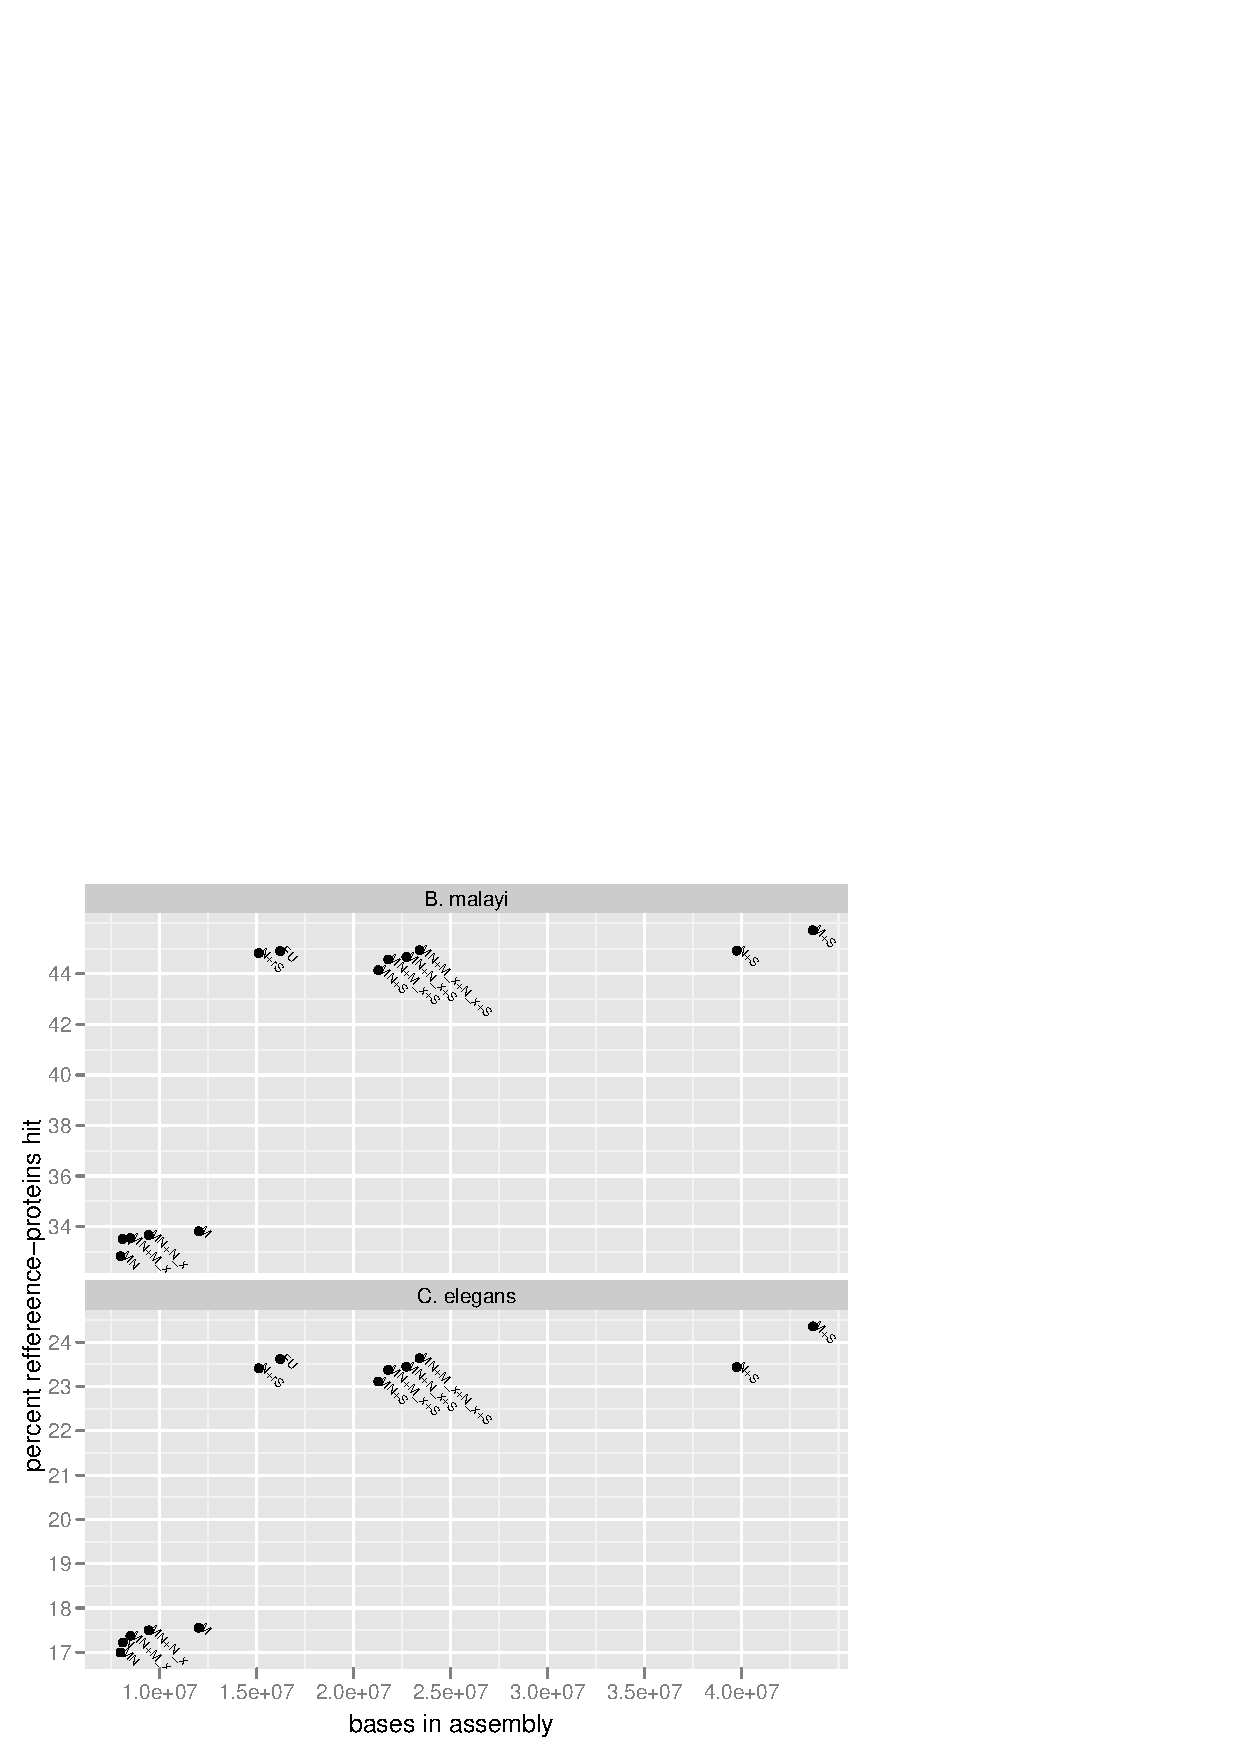
\includegraphics{Method-021}
\caption{Base-content and reference-transcriptome coverage in percent
  of proteins hit for different assemblies and assembly-combinations
  (for category-abrevations see Figure \ref{fig:basecov}).}
\label{fig:protcov}
\end{figure}

Considering the reference-database with any kind of coverage the
second-order assembly performed less preferable. Excluding singletons
it was covering similar numbers of database-proteins than the
Newber-assembly and and was outperformed by the Mira-assembly,
although the latter showed again to be least parsimonious. The same
general picture emerged from this analysis when singletons were
considered additionally. Newbler and second-order assemblies coverd
similar amounts of reference-data.

\begin{figure}[H]

\includegraphics{Method-022}
\caption{Base-content and reference-transcriptome coverage in percent
  of proteins coverd to at least 80\% of their length for different
  assemblies and assembly-combinations (for category-abrevations see
  Figure \ref{fig:basecov})}
\label{fig:prot80cov}
\end{figure}

When database-proteins covered for at least to 80\% of their length
are considered the second-order assembly showed it's superiority: Both
ex- and including singletons the second-order assembly outperformed
the first-order assemblies. Moderate gains in reference coverage were
made again for the addition of dubious single-assembler supported
second-order contigs. We give most weight in our analysis to these
results as in average longer correct contigs will allow finding the
highest number of putative full-lenth genes.

Given this evaluation we defined a ``minimal adequate'' assembly as the
subset of contigs of the second-order assembly supported by both
assemblers (labeled MN above). Given the performance of the singletons
\texttt{Newbler} reported. We defined a ``fullest-assembly'' as all
second-order contigs (including those supported by only one assembler)
plus the intersection of reported \texttt{Newbler}-singletons and
\texttt{Mira} singletons.

\section{Measurments on second-order assembly}

Based on the tracking of reads through the complicated assembly
process, we calculated the following statistics for each contig in the
second-order assembly.

\begin{itemize}
\item number of Mira and Newbler first-order contigs
\item number of reads through Mira and reads through Newbler
\item number of reads being split by Newbler in first-order assembly
\item number of read-split events in the first-order assembly (equals
  the sum of reads multiplied by number of contigs a read has been
  split into)
\item maximal number of first-order contigs a read in the contig has
  been split into during Newbler-assembly
\item the number of reads same-read-paires from the Newbler and Mira
  first order-assembly merged in a second order contig
\item cluster-id of the contig: All contigs ``connected'' by sharing
  reads (similar to the graph clustering reported in
  \cite{pmid21138572}). 
\item number of other second order contigs containing the same read
  (size of the cluster)
\end{itemize}





\subsection{Contig coverage}


\begin{Schunk}
\begin{Soutput}
null device 
          1 
\end{Soutput}
\begin{Soutput}
null device 
          1 
\end{Soutput}
\end{Schunk}

As well defined coverage-information is not readyly avaiable from the
output of this combined assembly aproach (although we followed
individual reads through the process) we inferred coverage by mapping
the reads used for assembly against the fullest assembly using ssaha2
\cite{pmid11591649} with parameters (-kmer 13 -skip 3 -seeds 6 -score
100 -cmatch 10 -ckmer 6 -output sam -best 1):

\begin{itemize}
\item mean per base coverage
\item mean unique per base coverage
\end{itemize}

The ratio of mean per base coverage and unique per base coverage (the
standard for assessing coverage) can be used as to asses the
redundancy of a contig.

\subsection{Example use of the contig-measurements}

Based on these measurements the emergence of a given contig from the
assembly process can be reconstructed. Table \ref{tab:ex-me} gives an
excerpt of the contig-measurements reported in additional-file
contig-data.csv. The example contigs are all from large
contig-clusters (cluster.size), where interpretation of the assembly
history is complicated, but not impossible:

% latex table generated in R 2.14.0 by xtable 1.6-0 package
% Fri Jan 13 08:45:09 2012
\begin{table}[ht]
\begin{center}
\begin{tabular}{rllll}
  \hline
 & Contig1047 & Contig10719 & Contig104 & Contig13672 \\ 
  \hline
reads\_through\_Newbler &   16 & 1351 &    0 &   14 \\ 
  reads\_through\_Mira &  26 & 651 & 135 &   0 \\ 
  Newbler\_contigs & 1 & 5 & 0 & 2 \\ 
  Mira\_contigs & 1 & 9 & 4 & 0 \\ 
  category & MN & MN & M\_n & N\_n \\ 
  num.new.split &    8 & 1314 &    0 &    0 \\ 
  sum.new.split &   16 & 2628 &    0 &    0 \\ 
  max.new.split & 2 & 2 & 0 & 0 \\ 
  num.SndO.pair &  13 & 644 &   0 &   0 \\ 
  cluster.id & CL62 & CL6 & CL176 & CL235 \\ 
  cluster.size & 24 & 18 &  5 &  5 \\ 
  coverage &   4.200342 & 267.495458 &  41.003369 &   2.920755 \\ 
  uniq\_coverage & 4.248960 & 7.425507 & 2.568000 & 1.196078 \\ 
   \hline
\end{tabular}
\caption{example table for assembly-measurements on contigs (as given in
                         contig-data.csv)}
\label{tab:ex-me}
\end{center}
\end{table}
\textbf{Contig1047} is in the well trusted MN category of contigs. It
consists of only one contig from each first-order assembly
(newbler\_contigs and mira\_contigs), each containing a set of reads
of moderate size: 16 from Newbler (reads\_through\_newbler) 26 from
Mira (reads\_through\_mira). 8 of the 16 reads Newbler used in its one
assembled contig were also assembled to a differnt Newbler-contig
(num.new.split). That each of the 8 reads was only appearing in one
other Newbler-contig is visible from the fact, that the number of
split events is 16 (sum.new.split) and the maximal number of splits
for one read is 2 (max.new.split). 13 (num.SndO.pair) same-read-pairs
from the tow different first-order assemblies were merged in this
second-order contig, leaving 3 (16-13) reads in Newbler-contigs and 13
(26-13) reads in Mira contigs, which all could potentially have ended
up in other contigs. The contig is in a cluster (CL62), which contains
in total 24 contigs (cluster.size). It has to be addmitted that the
whole graph-structure linking this 24 contigs can't be reconstructed
from this contig summary data. On the other hand the summary data
makes clear, from what source the links for cluster-affiliation have
resulted: In this case from 3 and 13 unlinked read-paires from both
first-order assemblies and 8 split-reads from Newbler-first order
contigs.

A comprehensive interpretation of the other example-contigs depicted
is left to the reader. It should just be remarked, that in case of
one-assembler supported contigs, all reads in that contig could
potentially be represented in other contigs, making average
cluster-size in these contigs bigger than in MN category.\\

One of the most interesting measurement calculated for each contig is
the cluster-membership and cluster-size. Such clusters can represent
close paralogs, duplicated genes, isoforms from alternative splicing
or allelic variants.

These measurements can be used in later analysis to e.g. reevaluate
the likelihood of misassembly in a given set of biologically relevant
contigs. All gene-sets mentioned later (in chapter the main text) were
thus, as a matter of routine, controlled for unusual patterns in the
contig meta-data.

\section{Finalising the fullest assembly set}
\label{sec:final-full-assembly}

In order to minimize the amount of sequence with artificially inferred
isoform-breakpoints we used the unique-mapping-information described
above to detect contigs and singletons not supported by any raw data
(reads). Table \ref{tab:cov.ex} gives a summary of these unsupported
data by contig-category. For all downstream-analysis we removed the
all well trusted MN-category-contigs no coverage and the contigs (and
singletons) from other categories having no unique coverage.

% latex table generated in R 2.14.0 by xtable 1.6-0 package
% Fri Jan 13 08:45:09 2012
\begin{table}[ht]
\begin{center}
\begin{tabular}{rrrrrrr}
  \hline
 & singletons & M\_1 & M\_n & MN & N\_1 & N\_n \\ 
  \hline
coverage == 0 & 546 &  34 &   2 &  36 & 158 &   0 \\ 
  unique coverage == 0 & 584 &  48 &   2 &  42 & 210 &   3 \\ 
   \hline
\end{tabular}
\caption{number of contigs with a coverage and unique-coverage of zero, inferred from mapping of raw reads, listed by contig-category}
\label{tab:cov.ex}
\end{center}
\end{table}
Thereby we reduced our dataset to 40,187 tentative unique genes
(TUGs), redefining the ``fullest assembly'' dataset. Based on the
above evaluation we decided to treat the MN-category of contigs as
high credibility assembly (highCA) and to subsume the M\_n, N\_n,
M\_1, N\_1 and \texttt{Newbler's} reported singletons as additional
low credibility assembly (lowCA).


%%%%%%%%%%%%%%%%%%%%%%%%%%%%%%%%%%%%%%%%%%%%%%%%%%%%%%%%%%%%%
%%                  The Bibliography                       %%
%%                                                         %%              
%%  Bmc_article.bst  will be used to                       %%
%%  create a .BBL file for submission, which includes      %%
%%  XML structured for BMC.                                %%
%%                                                         %%
%%                                                         %%
%%  Note that the displayed Bibliography will not          %% 
%%  necessarily be rendered by Latex exactly as specified  %%
%%  in the online Instructions for Authors.                %% 
%%                                                         %%
%%%%%%%%%%%%%%%%%%%%%%%%%%%%%%%%%%%%%%%%%%%%%%%%%%%%%%%%%%%%%


\bibliographystyle{/home/ele/bibtex/bmc_article.bst} % Style BST file
\newpage
\bibliography{/home/ele/bibtex/master.bib} % Bibliography file (usually '*.bib' )




\end{document}
